\providecommand{\main}{../../..}
\documentclass[\main/dresen_thesis.tex]{subfiles}
  \renewcommand{\thisPath}{\main/chapters/looselyPackedNS/structure}

\begin{document}
  \begin{figure}[tb]
    \centering
    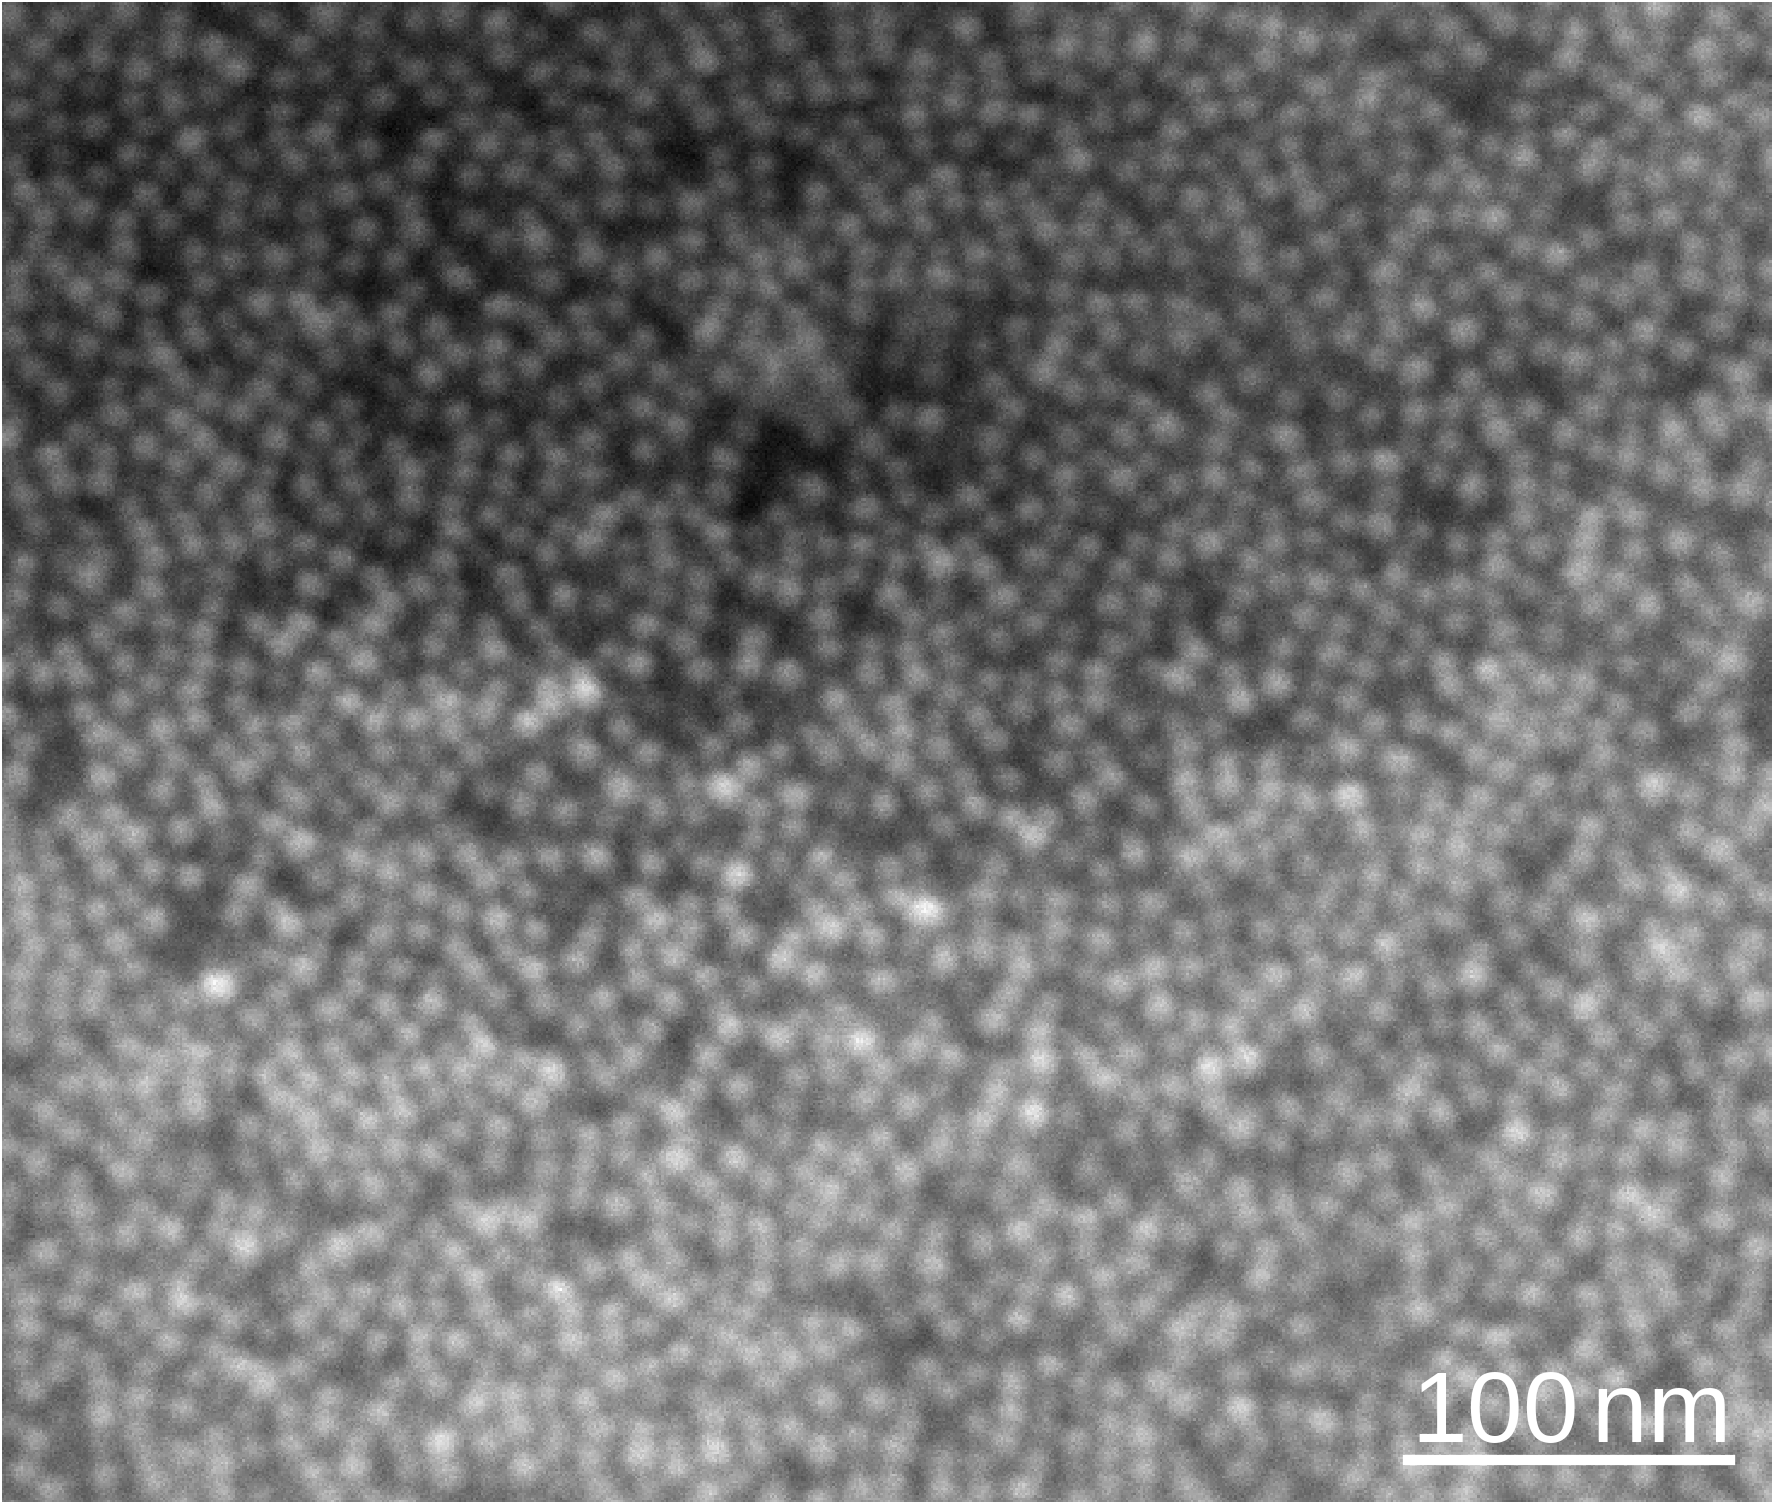
\includegraphics{looselyPackedNP_SEM_ES_S14_TopView}
    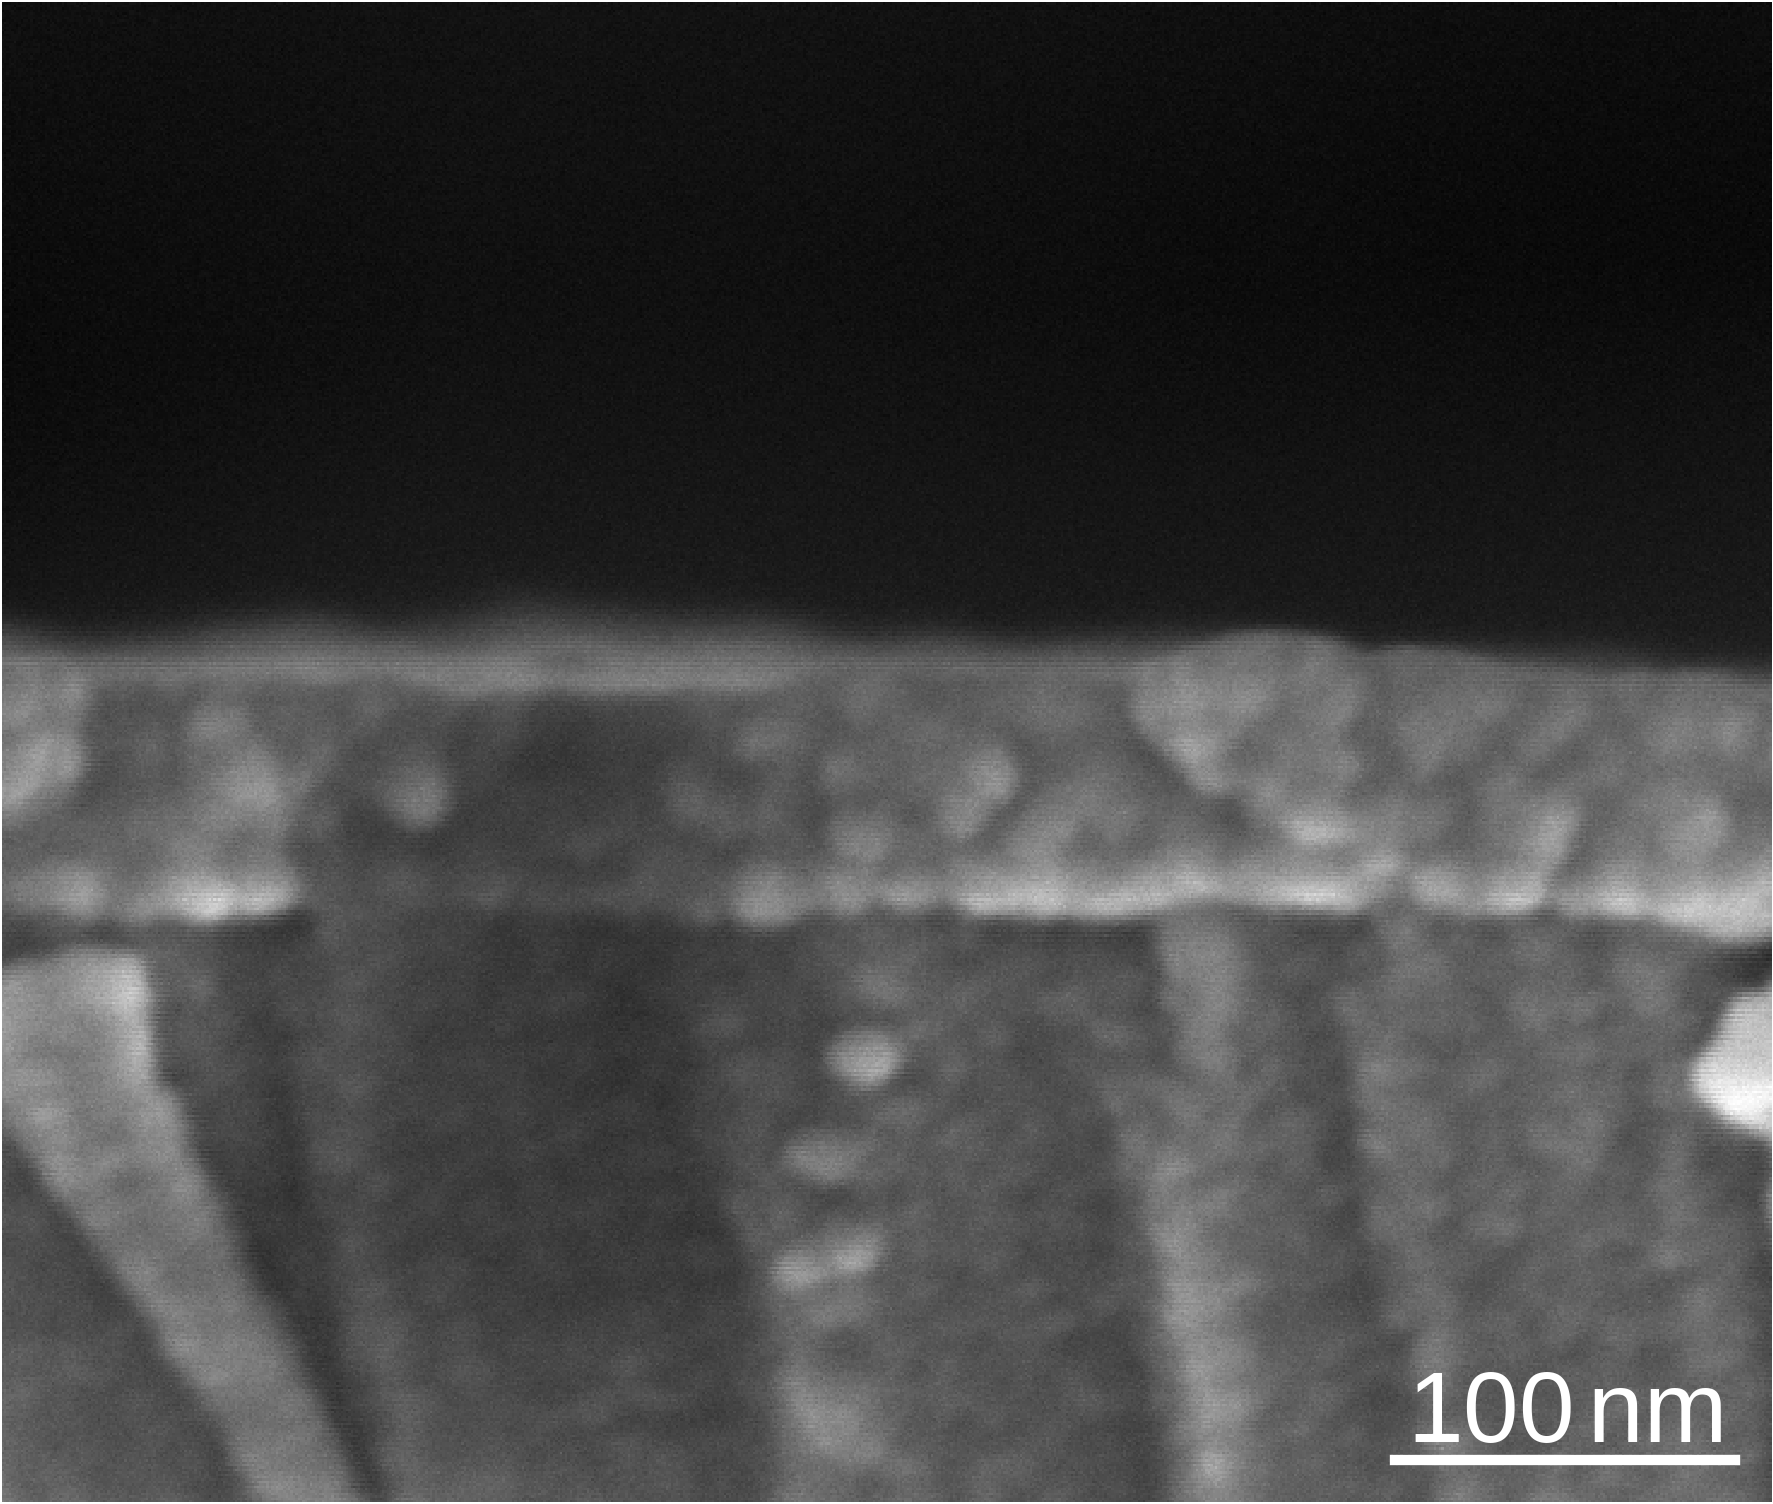
\includegraphics{looselyPackedNP_SEM_ES_S14}
    \caption{\label{fig:looselyPackedNP:nuclearStructure:sem}Scanning electron microscopy view of IOS-11 after spin coating on silicon from the top (left) and in cross section (right).}
  \end{figure}
  In a first step the spin-coated samples are studied structurally.
  By scanning electron microscopy (SEM), images of of the sample are taken at high magnification as shown in \reffig{fig:looselyPackedNP:nuclearStructure:sem}.
  The wafer was carefully broken into two pieces along a straight line to additionally study the cross sectional structure.
  On first glance, the homogeneous flat surface of the sample is visible in the cross section.
  In \reffig{fig:looselyPackedNP:nuclearStructure:semProjection}, the cross section is integrated along the vertical axis to estimate the average height of the sample at this local spot to $\approx 90 \unit{nm}$.

  The top view in \reffig{fig:looselyPackedNP:nuclearStructure:sem} shows no long range order among the nanoparticles and suggests that no dense packing is achieved through spin coating.
  Spheres that do not undergo any ordering process and are packed randomly have been studied extensively on the macroscopic scale \cite{Torquato_2000_IsRan} and it has been shown experimentally that the densest random close packing (RCP) lies in the order of $\approx 64 \, \%$.
  In a long range ordered crystalline structure, the closest packing spheres can achieve are the face-centered cubic and the hexagonal close-packed structure, which have a packing of $74 \, \%$.
  To study the packing of the nanoparticles, x-ray and neutron scattering provide non-destructive tools to quantify the order of the volume fraction across a large area of the sample.
  X-ray and neutron reflectometry is used to study the vertical structure of the sample, and grazing incidence small-angle x-ray scattering to study the lateral structure.

  \begin{figure}[tb]
    \centering
    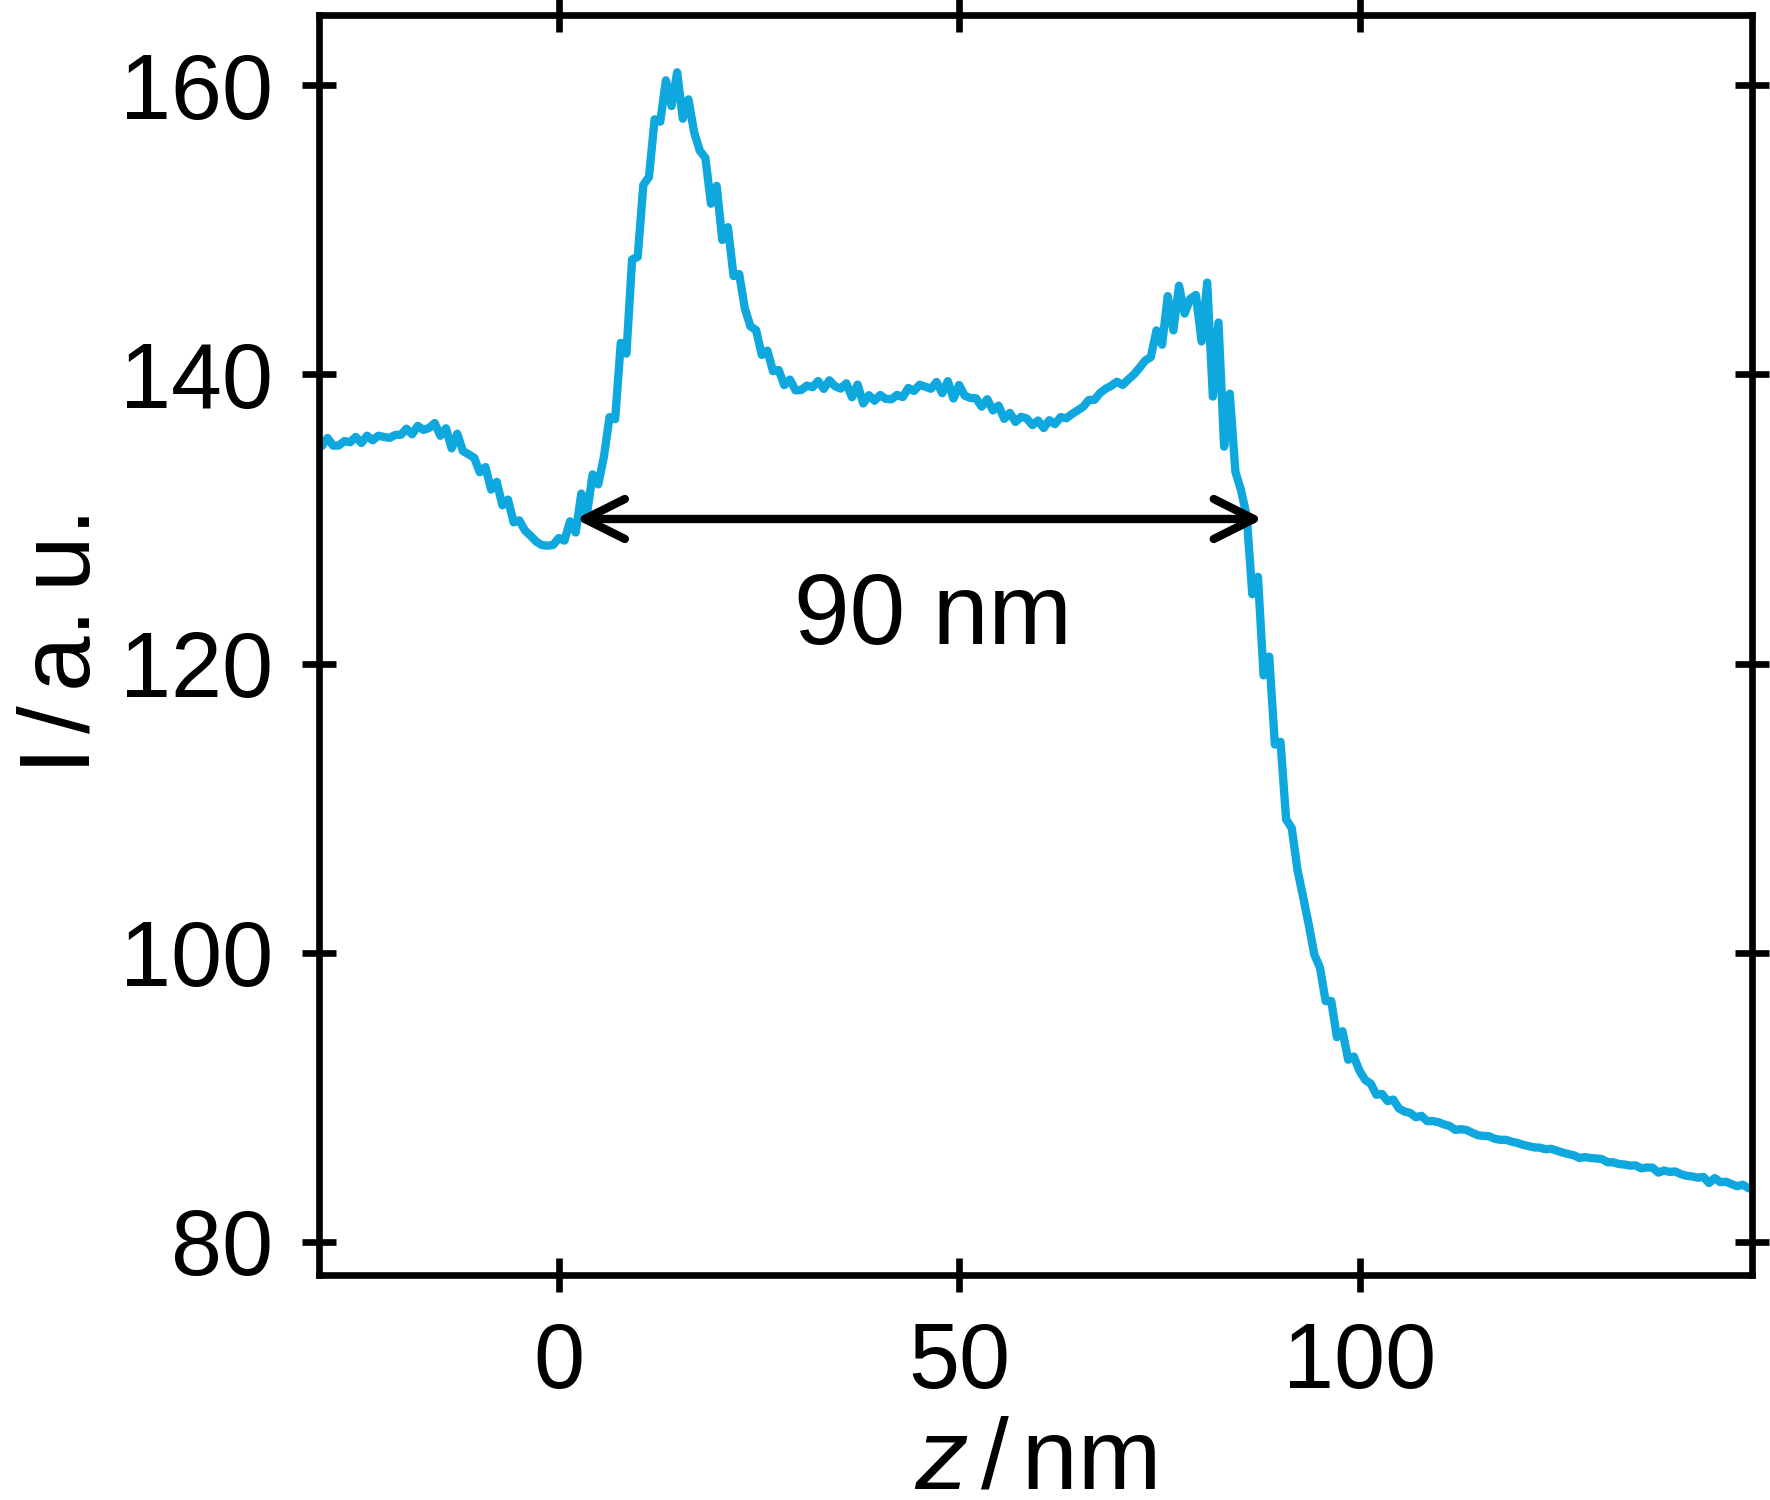
\includegraphics{looselyPackedNP_SEMprojection_ES_S14}
    \caption{\label{fig:looselyPackedNP:nuclearStructure:semProjection}Projection of the pixel intensity along the vertical axis from the cross sectional SEM shown in \reffig{fig:looselyPackedNP:nuclearStructure:sem}.}
  \end{figure}

  \begin{figure}[tb]
    \centering
    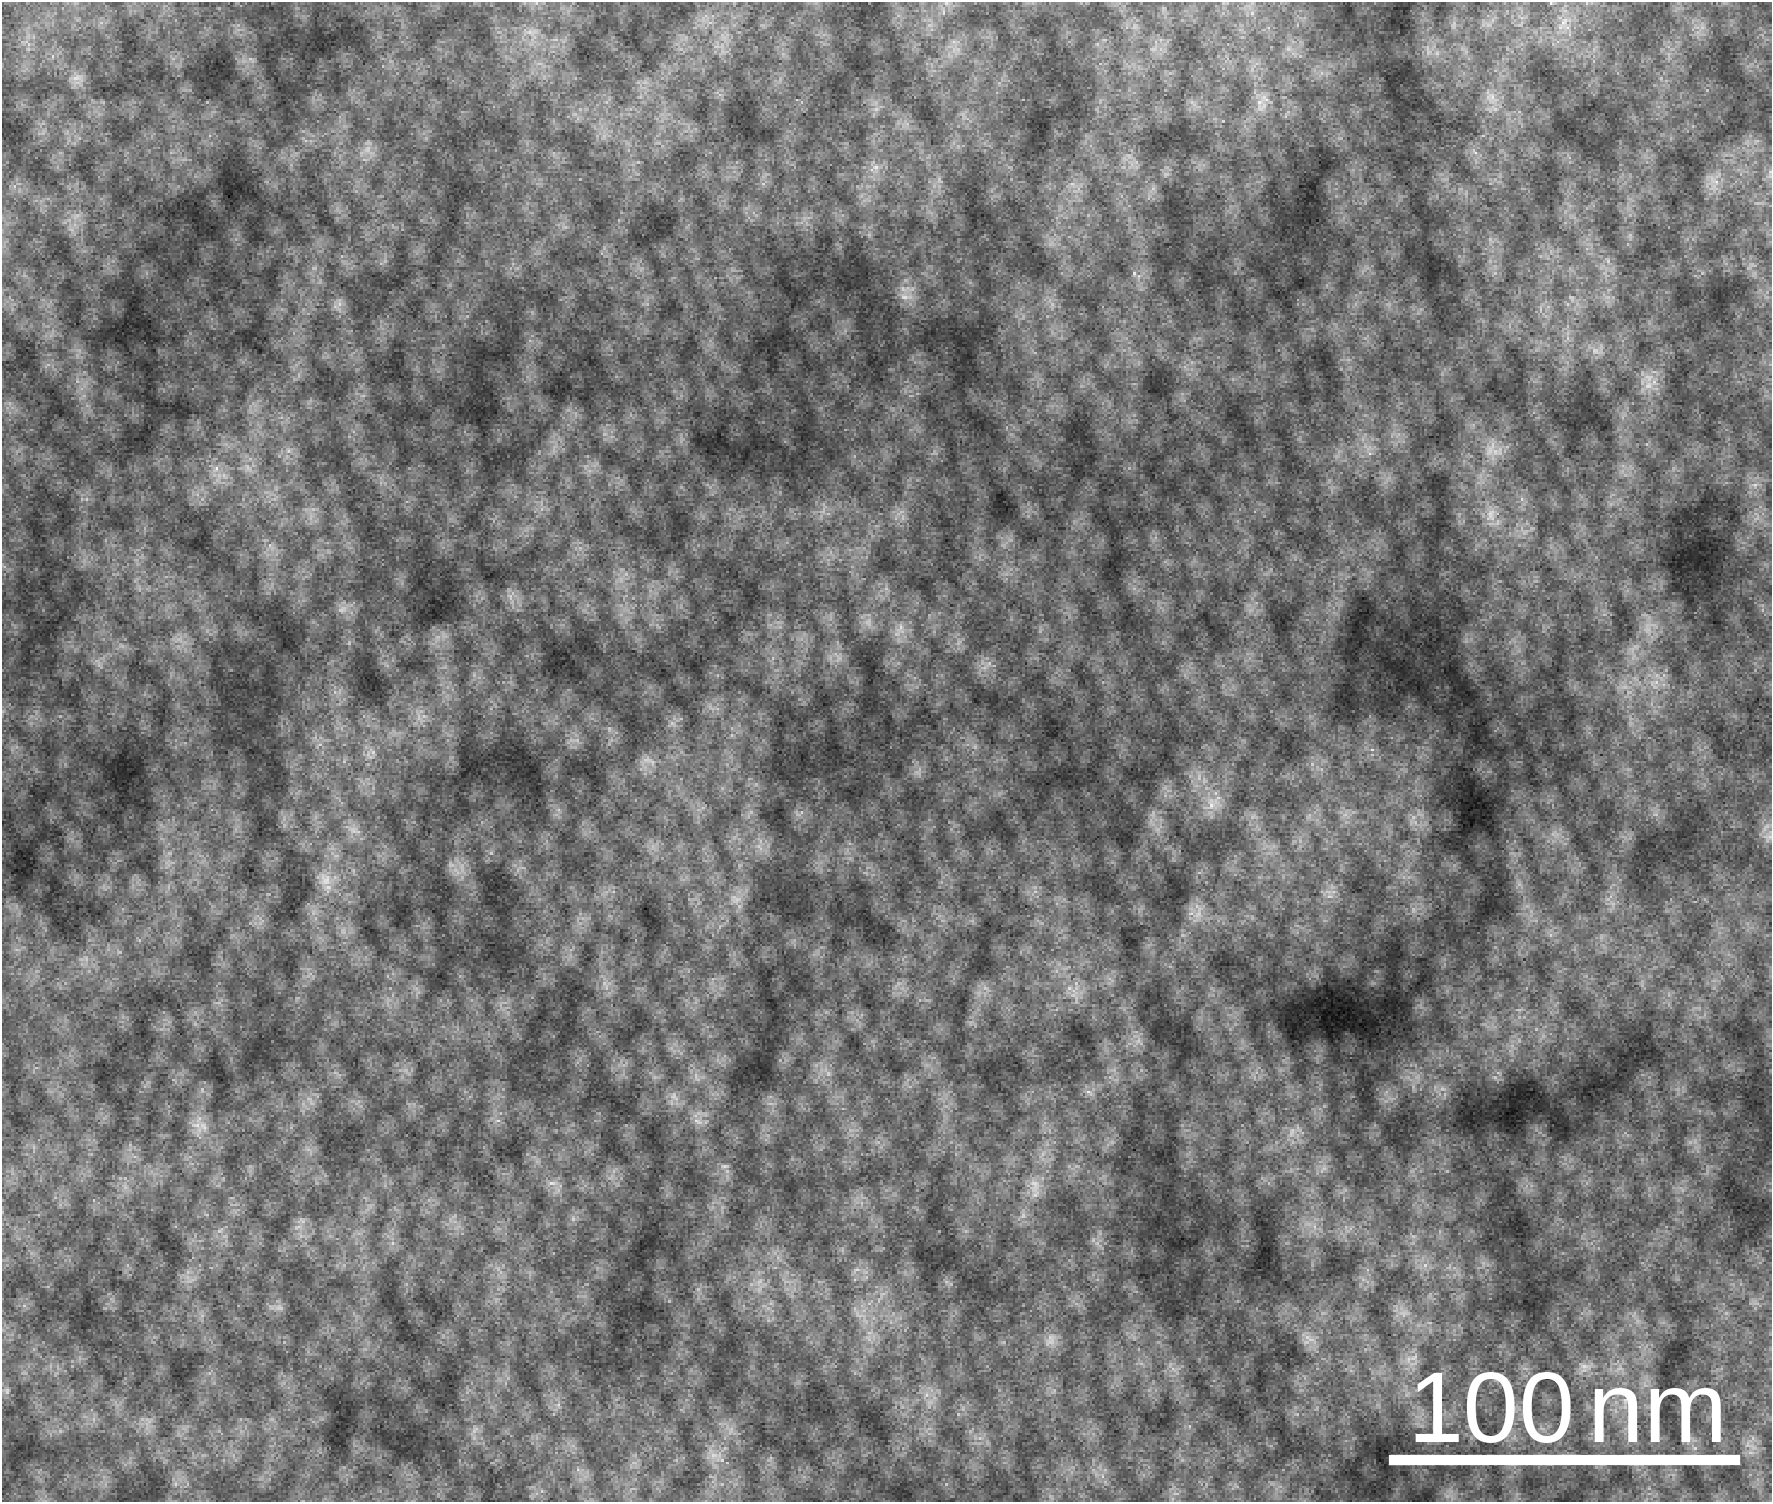
\includegraphics{looselyPackedNP_SEM_ES_S17_TopView}
    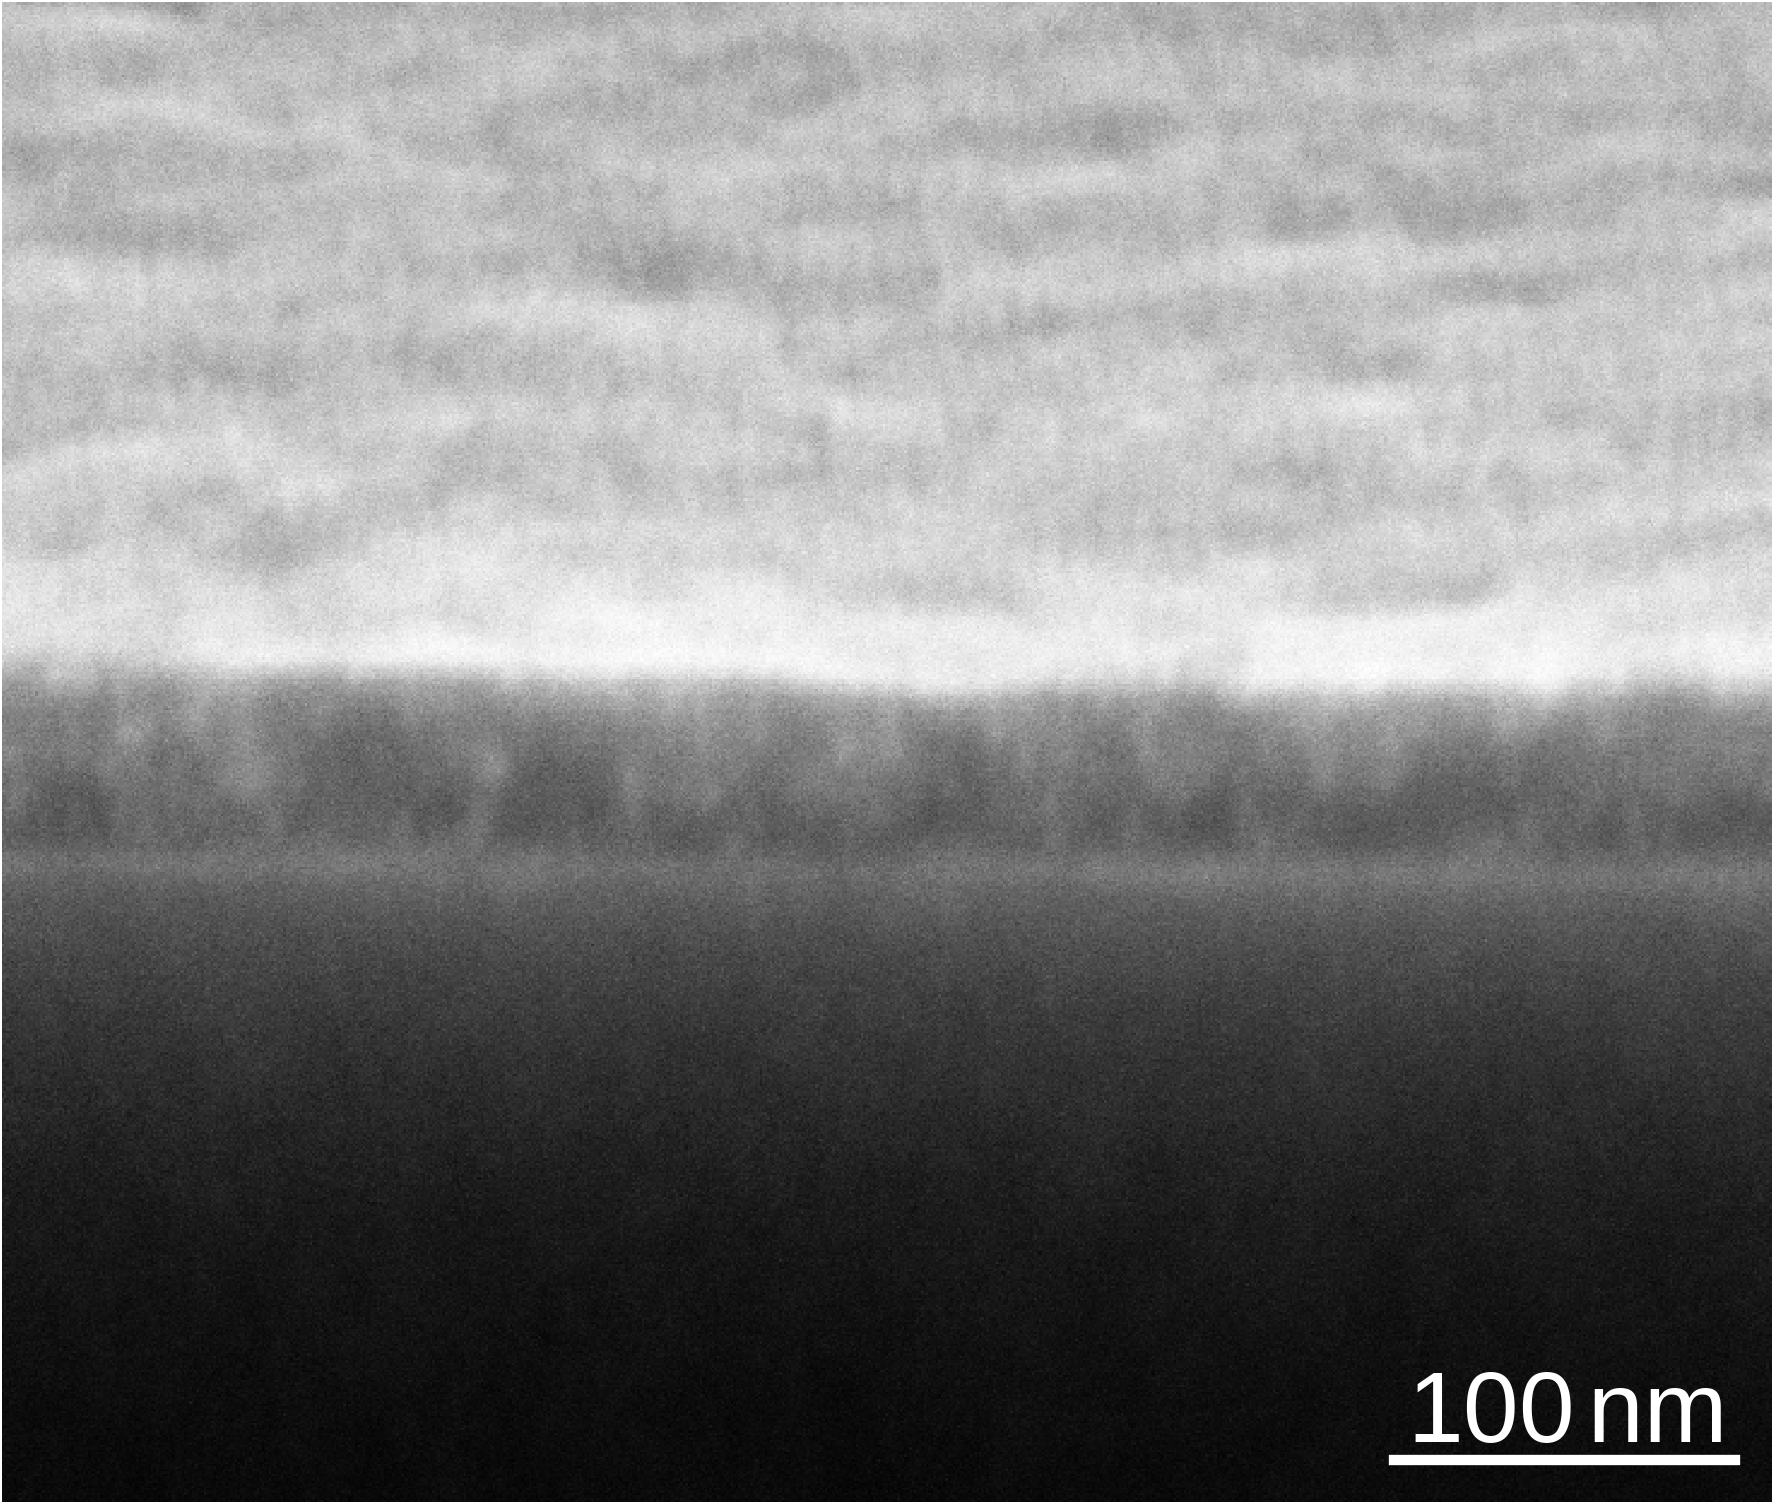
\includegraphics{looselyPackedNP_SEM_ES_S17}
    \caption{\label{fig:looselyPackedNP:nuclearStructure:semIOS7}Scanning electron microscopy view of IOS-7 from the top (left) and in cross section (right).}
  \end{figure}
\end{document}